\documentclass[tikz,border=0mm]{standalone}
\definecolor{iconblue}{RGB}{70,140,255}
\begin{document}
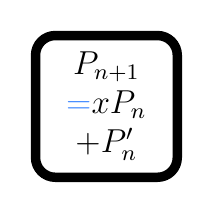
\begin{tikzpicture}[line width=1.2mm,line cap=round,line join=round]
  \useasboundingbox (-1,-1) rectangle (1,1);
  \draw[rounded corners=0.25cm] (-0.9,-0.9) rectangle (0.9,0.9);
  % Continue at the plus sign so the equation fits the standard square icon.
  \node[font=\large,inner sep=0pt] at (0,0.50) {$P_{n+1}$};
  \node[font=\large,inner sep=0pt] at (0,0.02)
    {$\textcolor{iconblue}{=}xP_n$};
  \node[font=\large,inner sep=0pt] at (0,-0.48) {$+P_n'$};
\end{tikzpicture}
\end{document}
